\documentclass{article}
\usepackage[accepted]{icml2018}
\usepackage{textcomp}
\usepackage{amsmath}
\usepackage{amssymb}
\usepackage{hyperref}
\usepackage{graphicx}
\usepackage{subcaption}
\usepackage{caption}
\usepackage{float}
\graphicspath{ {images/} }



\icmltitlerunning{Report Title}

\begin{document}

\twocolumn[
\icmltitle{E0:270 - Machine Learning - Understanding Generative Adversarial Networks}

\icmlsetsymbol{equal}{*}

\begin{icmlauthorlist}
\icmlauthor{Arpan Mangal}{dep1}
\icmlauthor{Rajarshi Banerjee}{dep2}
%\icmlauthor{Alphabetically}{dep1}
\end{icmlauthorlist}

\icmlaffiliation{dep1}{Department of Computer Science and Automation, Indian Insitute of Science, Bangalore}
\icmlaffiliation{dep2}{Department of Computer Science and Automation, Indian Insitute of Science, Bangalore}

\icmlcorrespondingauthor{Arpan Mangal}{arpanmangal@iisc.ac.in}
\icmlcorrespondingauthor{Rajarshi Banerjee}{rajarshib@iisc.ac.in}
%\icmlcorrespondingauthor{Alphabetically}{your@email.address}

\icmlkeywords{GAN, DCGAN, Generative networks, Adversarial training}

\vskip 0.3in
]

\printAffiliationsAndNotice{}

\begin{abstract}
Using  neural  networks  for  generating  synthetic data  is  a  difficult  task.    Generative  Adversarial Networks(GANs)  provide  an  interesting  approach to tackle this problem by pitting two networks to compete against each other.  However training a GAN is an extremely difficult task.  In this project we are trying to get an insight into the working of GANs and apply it to some interesting problem.
\end{abstract}

%\section{Introduction}
%\label{introduction}
%The PDF report should contain at most two pages excluding references and appendix and at most four pages including everything. Write about a subset of the following things that applies to your project:

%\begin{enumerate}
%	\item Problem Statement
%	\item Motivation
%	\item Literature Review
%	\item Model description
%	\item Dataset description
%	\item Preliminary Results
%	\item Future Work
%\end{enumerate}

\section{Problem statement}
\label{problem statement}
The aim of the project is to broadly survey a wide variety of GANs, to understand the various architectures, optimization techniques and/or other novel techniques used to better refine its training. We begin this exploratory journey from the humble beginnings of GAN \cite{ganpaper} and follow its various advancements and pitfalls \cite{towards} to quickly catapult ourselves to the bleeding edge of research on this topic \cite{wgan} only then to gently land on some of the aesthetic marvels produced by these networks \cite{cyclegan} and finally suggest a small yet peculiar mutation to one of its variants.
\section{Introduction}
\label{Introduction}
The advent of GAN came about with Ian Goodfellow's famous paper \cite{ganpaper}, and has enjoyed immense popularity ever since, at the heart of the matter lies a very simple formulation:
\[\min_G\max_DV(G,D)=\mathbb{E}_{x\sim p_{data}(x)}[\log D(x)] \]
\[\quad \quad \quad \quad \quad \quad \quad \quad + \quad \mathbb{E}_{z\sim p_z(z)}[\log (1-D(G(z)))]\]
Where $p_z(z)$ is the prior of the input noise variable, $p_{data}(x)$ is the unknown data distribution from which the training samples (are assumed to) come from. $G$ and $D$ are the generator and discriminator networks respectively.\newline
The paper proves that when the discriminator $D$ is trained to optimality, training the generator $G$ minimizes $JSD(P_{data}||p_{g})$, i.e. the Jensen---Shannon divergence between the model\textquotesingle s distribution and the data generating process.

\section{Deep Convolution GANs}
\label{deep convolution GANs}
Out of the many variants in GAN architecture, the deep convolution GAN (DCGAN) is one of the most simple architecture that is widely used, \cite{dcgan} also provides a list of guidelines to follow that has been empirically know to give good quality outputs. The guidelines suggested by the paper are:
\begin{itemize}
    \item Replace any pooling layers with strided convolutions (discriminator) and fractional-strided
convolutions (generator).
    \item Use batchnorm in both the generator and the discriminator.
    \item Remove fully connected hidden layers for deeper architectures.
    \item Use ReLU activation in generator for all layers except for the output, which uses Tanh.
    \item Use LeakyReLU activation in the discriminator for all layers.
\end{itemize}
%\begin{figure}[h!]
%    \centering
%    \includegraphics[width=6cm]{DCGAN.png}
%    \caption{The DCGAN generator architecture as suggested by the paper}
%    \label{fig:my_label}
%\end{figure}
\section{Problems training a GAN}
\label{problems training a GAN}
\begin{enumerate}
    \item \textbf{Hard to achieve Nash equilibrium:} \cite{improved_training} discussed the problem with GAN’s gradient-descent-based training procedure. Two models are trained simultaneously to find a Nash equilibrium to a two-player non-cooperative game, with each model updating its cost independently with no respect to another player in the game does not guarantee a convergence.
    \item \textbf{Low-dimensional supports:} \cite{towards} discussed the problem of the supports of $p_{data}$ and $p_g$ lying on low dimensional manifolds and how it contributes to the instability of GAN training.\newline
    The dimensions of many real-world datasets, as represented by $p_{data}$, only appear to be artificially high.\newline
    Because both $p_g$ and $p_{data}$ rest in low dimensional manifolds, they are almost certainly gonna be disjoint. When they have disjoint supports, we are always capable of finding a perfect discriminator that separates real and fake samples 100\% correctly.
    \item \textbf{Vanishing gradients:} When the discriminator is perfect, we are guaranteed with $D(x)=1,\forall x\in p_{data}$ and $D(x)=0,\forall x\in p_g$. Therefore the loss function for the generator falls to zero and we end up with no gradient to update the loss during learning iterations
    \begin{figure}[h!]
        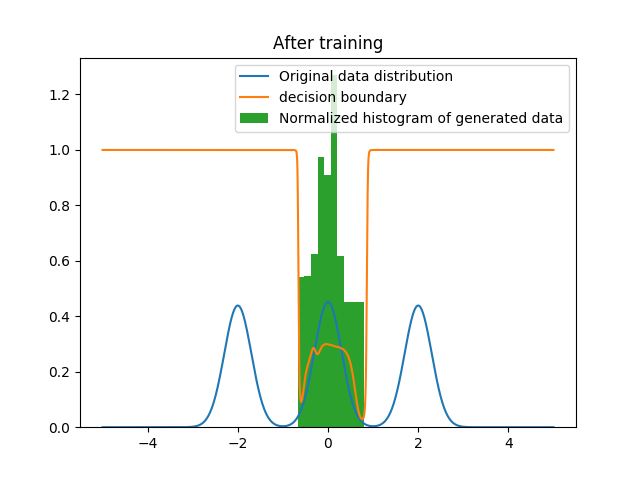
\includegraphics[width=7cm]{d_more_than_g.png}
        \caption{Effect on output distribution when discriminator is trained to optimality. Here the generator cannot learn the entire distribution as the discriminator is too powerful }
        \label{fig:0}
    \end{figure}
    \item \textbf{Mode Collapse:} During the training, the generator may collapse to a setting where it always produces same outputs. This is a common failure case for GANs, commonly referred to as \textbf{Mode Collapse}. Even though the generator might be able to trick the corresponding discriminator, it fails to learn to represent the complex real-world data distribution and gets stuck in a small space with extremely low variety.
    \begin{figure}[h!]
        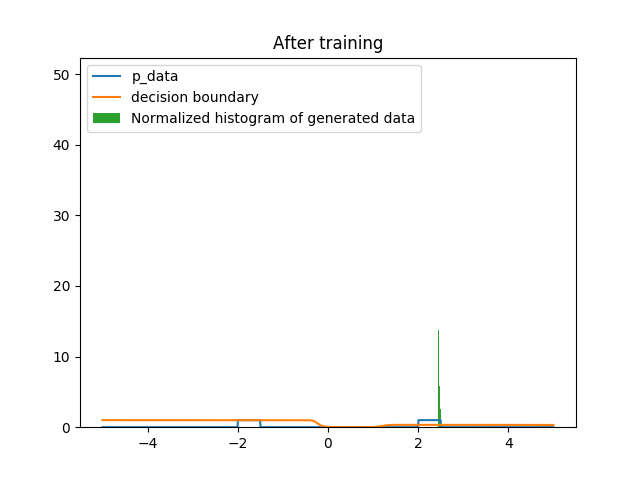
\includegraphics[width=7cm]{helevetica.png}
        \caption{Effect on output distribution on training it on a mixture of two uniform distribution where generator is trained much more than the discriminator, here the output distribution collapses to a very small range. This scenario is known as mode collapse or helvetica }
        \label{fig:2}
    \end{figure}
    \item \textbf{Lack of a proper evaluation metric:} Generative adversarial networks are not equipped with a good objective function that can inform us the training progress. Without a good evaluation metric, it is like working in the dark. No good sign to tell when to stop; No good indicator to compare the performance of multiple models.
\end{enumerate}
\section{Wasserstein GAN }
As we mentioned, training of standard GAN is very unstable and slow. Main problem is with the loss metric i.e. JS divergence, which is not continuous and differentiable everywhere. Due to which, it's very difficult to maintain balance between generator's and discriminator's training. If we train discriminator less, then our generator will not get true feedback to update, and on the other hand if we train it to optimality, we will hit vanishing gradient problem.\\
Recently there is a interest in the paper \cite{wgan}, which claims to solve these problem. In WGAN, we use Earth-Mover(EM) distance as loss metric. EM distance under mild assumptions is continuous and differentiable everywhere. Assumption is that mapping of \textbf{$\theta \rightarrow g(\theta$)} (where $\theta$ is generator's parameter) is continuous and \textbf{g} is locally Lipschitz, which holds in case of GAN's because g is multi-layer feed forward network.\\
It has following advantages over standard GAN's : 
\begin{enumerate}
\item We can train our critic (same as discriminator) to optimality without vanishing gradient problem, therefore leads to correct feedback to generator and leads to stability.
\item EM distance is very meaningful loss metric i.e. correlates well with the quality of the generated samples.
\item The  mode dropping phenomenon that is typical in GANs is also  drastically reduced (empirically).
\end{enumerate}


\subsection{WGAN Formulation}
The EM distance used here (also called as Wasserstein distance.
\[
W(p_r, p_g) = \inf_{\gamma \sim \Pi(p_r, p_g)} E_{(x, y) \sim \gamma}[\| x-y \|]
\]
where $\gamma \in \Pi(p_r, p_g)$, is the set of all distributions whose marginals are $p_r$ and $p_g$ respectively.\\

In above formulation we have $\inf$ over all valid $\gamma$ which is intractable. In paper, author cleverly convert it into $\sup$ using Kantorovich-Rubinstein duality. Intutively, it can be seen as dual of linear program (refer to this blog).\\

Let  \(\mathbf{\Gamma} = \gamma(x,y)\) and \(\mathbf{D} = \Vert x - y \Vert\) , with \( \mathbf{\Gamma}, \mathbf{D} \in \mathbb{R}^{l \times l} \)
\[\mathrm{EMD}(P_r, P_\theta) = \inf_{\gamma \in \Pi} \, \langle \mathbf{D}, \mathbf{\Gamma} \rangle_\mathrm{F} \]
 where, \( \langle , \rangle_\mathrm{F}\) , is the Frobenius inner product (sum of all the element-wise products).
 \\
This can be thought as a minimization Linear program under the constraint the \(P_r\) and \(P_\theta\) are marginals of \(\gamma\).\\\\Since, Infimium in this problem is intractable, we can solve its dual.
 \[\mathrm{EMD}(P_r, P_\theta) = \sup_{\lVert f \lVert_{L \leq 1}} \ \mathbb{E}_{x \sim P_r} f(x) - \mathbb{E}_{x \sim P_\theta} f(x)\]
 \\
 Suppose this function f comes from a family of K-Lipschitz continuous functions, \(\{ f_w \}_{w \in W}\), parameterized by w. In the modified WGAN, the “discriminator” model is used to learn w to find a good \(f_w\) and the loss function is configured as measuring the Wasserstein distance between \(p_r\) and \(p_g\).

\[L(p_r, p_g) = W(p_r, p_g) = \max_{w \in W} \mathbb{E}_{x \sim p_r}[f_w(x)] \]
\[\quad \quad \quad \quad \quad \quad \quad \quad \quad \quad- \quad \mathbb{E}_{z \sim p(z)}[f_w(g_\theta(z))]\]Thus the “discriminator” is not a direct critic of telling the fake samples apart from the real ones anymore. Instead, it is trained to learn a K-Lipschitz continuous function to help compute Wasserstein distance. As the loss function decreases in the training, the Wasserstein distance gets smaller and the generator model’s output grows closer to the real data distribution.

%\section{Dataset description}
%\label{dataset description}
%Till now the datasets on which we have trained our GANs are: MNIST and LSUN outdoor church datasets.
\section{Cycle GANs}
\label{Cycle GAN}
\begin{figure}[h!]
        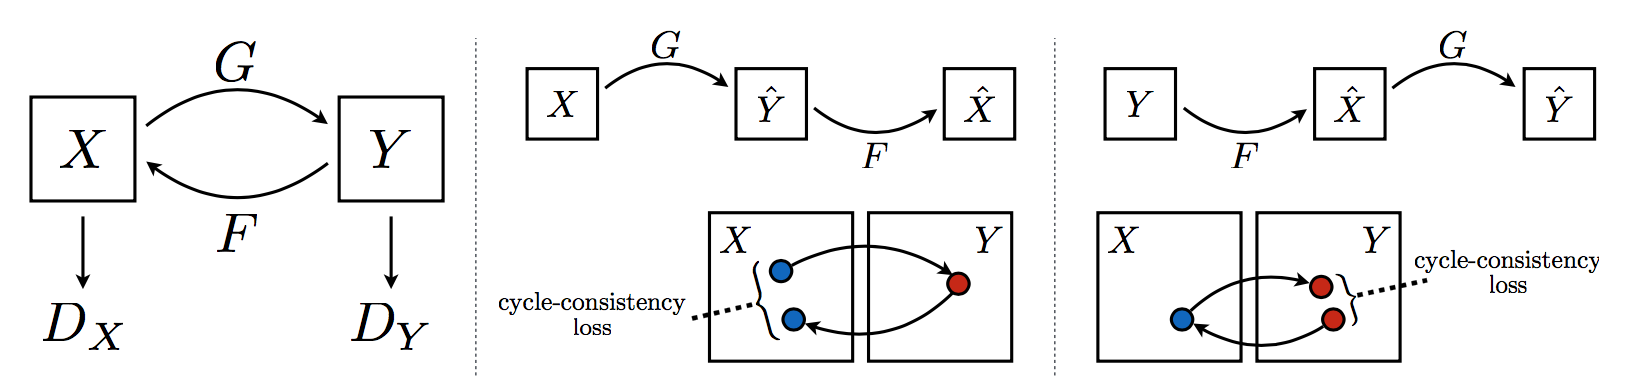
\includegraphics[width=8.5cm]{Cycle_GAN_idea.png}
        \caption{ $G$ and $F$ are the generator networks that convert $X$ to $Y$ and $Y$ to $X$ respectively, with $D_X$ and $D_Y$ being the corresponding discriminators}
        \label{fig:2}
\end{figure}
Next we looked into some the practical applications of GANs in image transformations as discussed in the paper \cite{cyclegan}.\newline
In a Cycle GAN we train two GANs in parallel to convert data from domain X to domain Y and vice-versa, and also add another loss called the cycle consistency loss that acts as the regularizer of the network.
\[\mathcal{L}_{cyc}(G,F)=\mathbb{E}_{x\sim p_{data}(x)}[||F(G(x)) - x||_1]\]
\[\quad\quad\quad\quad\quad\quad+\quad\mathbb{E}_{y\sim p_{data}(y)}[||G(F(x)) - y||_1]\]
\[\mathcal{L}(G,F,D_X,D_Y) = \mathcal{L}_{GAN}(G,D_Y,X,Y)\]
\[\quad\quad\quad\quad\quad\quad\quad+\quad\mathcal{L}_{GAN}(F,D_X,X,Y)\]
\[\quad\quad\quad\quad+\quad\lambda\mathcal{L}_{cyc}(G,F)\]

\subsection{Proposed modification to the Cycle GAN architecture}
\label{propsed modification to cycle GAN architecture}
The architecture proposed in \cite{cyclegan} is based on \cite{perceptual_loss}. We propose a simple modification to this architecture: \newline
Rather than using two separate generators $G$ and $F$ we can use a common encoder and two decoders for each of the domains. The original architecture of the generator is a pair of convolution networks followed by 6 residual blocks and finally a pair of transposed convolution networks for upsampling. Our implementation uses a common encoder for both the GANs that consists of the first two convolution networks followed by 3 residual blocks, and two decoders for domain $X$ and $Y$ consisting of 3 residual blocks followed by 2 transposed convolution layers. It is essentially a partition of the original architecture into an encoder and a decoder.\newline
This resulted in a much smaller size of the overall network and the training speed increased by more than a factor of 2, however the image quality was relatively poor.

\section{Experiments}
\label{results}
\subsection{Dataset description}
We used the MNIST dataset \cite{mnist} and LSUN outdoor church dataset \cite{yu15lsun} for training our DCGAN and WGAN.
We used the datasets 'monet$\leftrightarrow$photo' , 'winter$\leftrightarrow$summer' as described in \cite{cyclegan} for training the Cycle GAN and our modified variant of it.
\subsection{Code}
\url{https://github.com/Evil-Incorporated/basic-gans}
\subsection{Results}
\begin{figure}[H]
    \centering
    \begin{subfigure}{.125\textwidth}
        \centering
        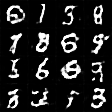
\includegraphics[width=.9\linewidth]{GAN_epoch001.png}
        \caption{Epoch 1}
    \end{subfigure}%
    \begin{subfigure}{.125\textwidth}
        \centering
        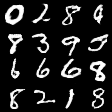
\includegraphics[width=.9\linewidth]{GAN_epoch010.png}
        \caption{Epoch 10}
    \end{subfigure}%
    \begin{subfigure}{.125\textwidth}
        \centering
        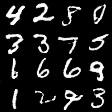
\includegraphics[width=.9\linewidth]{GAN_epoch020.png}
        \caption{Epoch 20}
    \end{subfigure}%
    \begin{subfigure}{.125\textwidth}
        \centering
        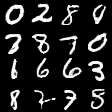
\includegraphics[width=.9\linewidth]{GAN_epoch025.png}
        \caption{Epoch 25}
    \end{subfigure}
    \caption{DCGAN generator output on MNIST Dataset}
    \label{fig:my_label}
\end{figure}
\begin{figure}[H]
    \centering
    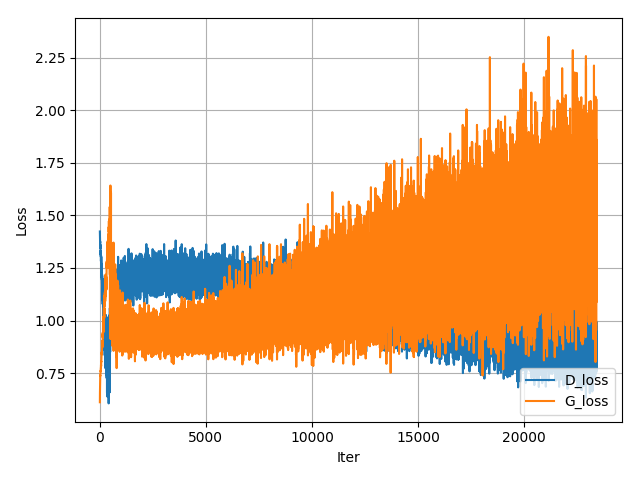
\includegraphics[width=0.9\linewidth]{GAN_loss.png}
    \caption{Discriminator loss $D_{loss}$ and Generator loss $G_{loss}$ on the MNIST dataset, this also goes to illustrate the fact that there is no proper evaluation metric in the standard GAN}
    \label{fig:my_label}
\end{figure}
\begin{figure}[H]
    \centering
    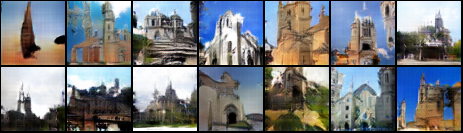
\includegraphics[width=0.9\linewidth]{display_sample_LSUN_DCGAN.png}
    \caption{Output of DCGAN on LSUN outdoor church dataset after 25 epochs}
    \label{fig:my_label}
\end{figure}
\begin{figure}[H]
    \centering
    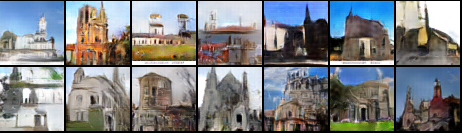
\includegraphics[width=0.9\linewidth]{display_WGAN_LUSN.png}
    \caption{Output of WGAN with DCGAN architecture on LSUN outdoor church dataset after 25 epochs}
    \label{fig:my_label}
\end{figure}
\begin{figure}[H]
    \centering
    \begin{subfigure}{.112\textwidth}
        \centering
        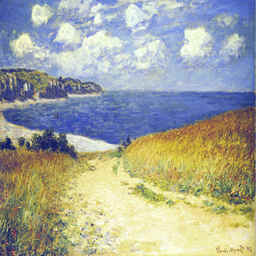
\includegraphics[width=\linewidth]{00010.jpg}
    \end{subfigure}%
    \begin{subfigure}{.112\textwidth}
        \centering
        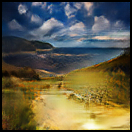
\includegraphics[width=\linewidth]{0001.png}
    \end{subfigure}\hspace{.010\textwidth}%
    \begin{subfigure}{.112\textwidth}
        \centering
        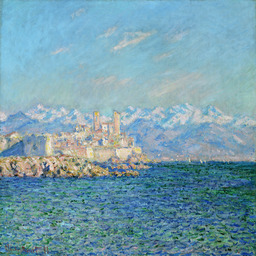
\includegraphics[width=\linewidth]{00020.jpg}
    \end{subfigure}%
    \begin{subfigure}{.112\textwidth}
        \centering
        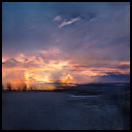
\includegraphics[width=\linewidth]{0002.png}
    \end{subfigure}
    
    \begin{subfigure}{.112\textwidth}
        \centering
        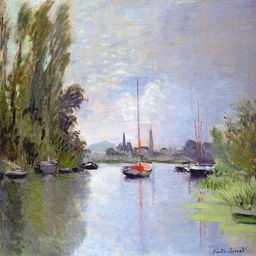
\includegraphics[width=\linewidth]{00030.jpg}
    \end{subfigure}%
    \begin{subfigure}{.112\textwidth}
        \centering
        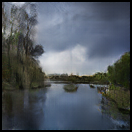
\includegraphics[width=\linewidth]{0003.png}
    \end{subfigure}\hspace{.010\textwidth}%
    \begin{subfigure}{.112\textwidth}
        \centering
        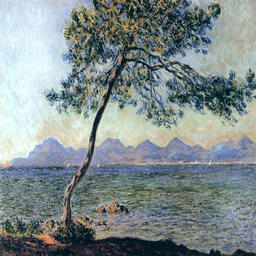
\includegraphics[width=\linewidth]{00040.jpg}
    \end{subfigure}%
    \begin{subfigure}{.112\textwidth}
        \centering
        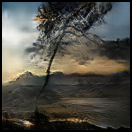
\includegraphics[width=\linewidth]{0004.png}
    \end{subfigure}
    
    \begin{subfigure}{.112\textwidth}
        \centering
        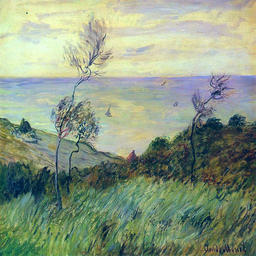
\includegraphics[width=\linewidth]{00170.jpg}
    \end{subfigure}%
    \begin{subfigure}{.112\textwidth}
        \centering
        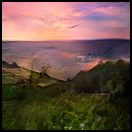
\includegraphics[width=\linewidth]{0017.png}
    \end{subfigure}\hspace{.010\textwidth}%
    \begin{subfigure}{.112\textwidth}
        \centering
        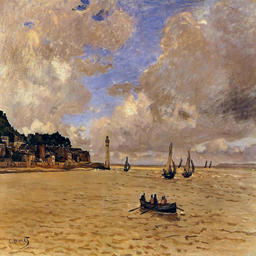
\includegraphics[width=\linewidth]{00360.jpg}
    \end{subfigure}%
    \begin{subfigure}{.112\textwidth}
        \centering
        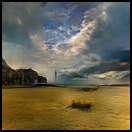
\includegraphics[width=\linewidth]{0034.png}
    \end{subfigure}
    
    \begin{subfigure}{.112\textwidth}
        \centering
        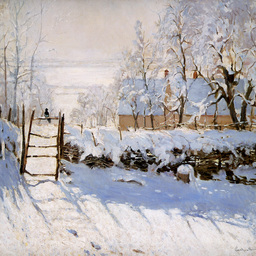
\includegraphics[width=\linewidth]{00855.jpg}
        \caption{Input}
    \end{subfigure}%
    \begin{subfigure}{.112\textwidth}
        \centering
        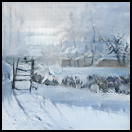
\includegraphics[width=\linewidth]{0075.png}
        \caption{Ouput}
    \end{subfigure}\hspace{.010\textwidth}%
    \begin{subfigure}{.112\textwidth}
        \centering
        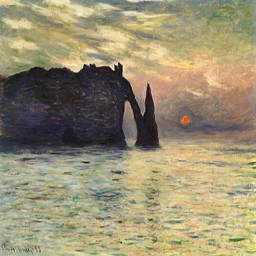
\includegraphics[width=\linewidth]{00860.jpg}
        \caption{Input}
    \end{subfigure}%
    \begin{subfigure}{.112\textwidth}
        \centering
        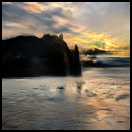
\includegraphics[width=\linewidth]{0076.png}
        \caption{Ouput}
    \end{subfigure}
    \caption{Cycle GAN output of Monet paintings to photorealistic pictures}
    \label{fig:my_label}
\end{figure}

\begin{figure}[H]
    \centering
    \begin{subfigure}{.165\textwidth}
        \centering
        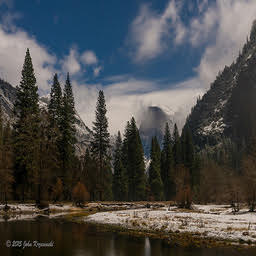
\includegraphics[width=0.75\linewidth]{Input_1.jpg}
    \end{subfigure}%
    \begin{subfigure}{.165\textwidth}
        \centering
        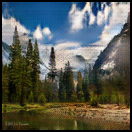
\includegraphics[width=0.75\linewidth]{output_1_cycle_gan.png}
    \end{subfigure}%
    \begin{subfigure}{.165\textwidth}
        \centering
        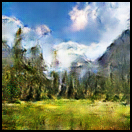
\includegraphics[width=0.75\linewidth]{output_1_modified_cycle_gan.png}
    \end{subfigure}
    
    \begin{subfigure}{.165\textwidth}
        \centering
        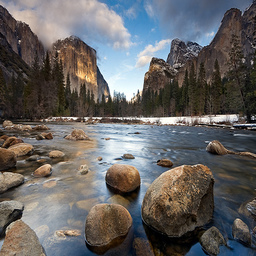
\includegraphics[width=0.75\linewidth]{Input_2.jpg}
        \caption{}
    \end{subfigure}%
    \begin{subfigure}{.165\textwidth}
        \centering
        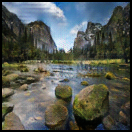
\includegraphics[width=0.75\linewidth]{output_2_cycle_gan.png}
        \caption{}
    \end{subfigure}%
    \begin{subfigure}{.165\textwidth}
        \centering
        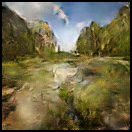
\includegraphics[width=0.75\linewidth]{output_2_modified_cycle_gan.png}
        \caption{}
    \end{subfigure}
    
    \caption{Winter to summer conversion on the 'summer$\leftrightarrow$winter' dataset. (a) Input (b) Cycle GAN output (c) Fused encoder Cycle GAN output}
    \label{fig:my_label}
\end{figure}

\section{Conclusion}
In this paper we have presented a brief overview of the various aspects of GANs we have explored, by no means was this an exhaustive search and there are many more variants of GANs that we did not include in the project. More importantly we do not yet know whether our modification to the Cycle GAN is capable of generalizing to other domains, however we believe that it would be fruitful to direct our attention towards it in the future.



%\section{Future Work}
%\label{future work}
%We next intent to implement the Wasserstein loss function in our GANs to see how the generated image quality changes, along with tuning some hyper parameters, we also intend to look into other practical applications that can be performed using GANs. 

%Good fellow : Basic structure/theory behind of GAN. Loss functions useed when both discriminator and generator are MLP/NN

%Towards understanding: Theoritically proved why traing GAN is hard because of vanishing gradient. Distributions Pr(true) and Pg(generated) are not continuos or have disjoint supports leads of max out of divergenge. Noise is added to true distribution to make it continuos.
%We have also reviwed DCGAN architecture, WGAN arcitecture.


%Preliminary results.
%We have iumplemented athe availabe codes for
%1. 1-D gaussian
%2. MNIST dataset
%3. Lsun dataset
%observations :
% (i) if we traine D more, genreate didnt uodated
% (ii) that modelas are sensitive to parametrs
%(iii) if mixture of gaussian
%(iv) unstable
%(v) sensitive of z-distribution



%You can additionally provide anything else that is relevant to your project but is not present in the list given above. 

%You can create various sections/subsections etc. to organise your report as per the need. Use \texttt{biblio.bib} file to provide references. The references should be provided by using cite keyword \cite{langley00}.

%You can contact your project mentor if you have any confusion.


%%%%%%%%%%%%%%%%%%%%%%%%%%%%%%%%%%%%%%%%%%%%%%%%%%%%%%%%%%%%%%%%%%%%%%%%%%%%%%%
\newpage
\clearpage
\bibliography{biblio}
\bibliographystyle{icml2018}


%%%%%%%%%%%%%%%%%%%%%%%%%%%%%%%%%%%%%%%%%%%%%%%%%%%%%%%%%%%%%%%%%%%%%%%%%%%%%%%
% Remove this part if you are not using an Appendix. Appendix is ungraded. The
% reader may wish to ignore the appendix altogether. Write everything that you
% think is important in the main report text only.

%\appendix
%\section{Optional Appendix (Ungraded)}
%Remove this part if you are not using an Appendix. Appendix is ungraded. The
%reader may wish to ignore the appendix altogether. Write everything that you
%think is important in the main report text only.

%%%%%%%%%%%%%%%%%%%%%%%%%%%%%%%%%%%%%%%%%%%%%%%%%%%%%%%%%%%%%%%%%%%%%%%%%%%%%%%

\end{document}